\section{Análisis del proceso actual}\label{sec:analisis-proceso-actual}

Para poder determinar el flujo del sistema se deben analizar los procesos actuales del conjunto habitacional, para ello se debe identificar los actividades que se llevan a cabo en el conjunto habitacional, los actores que intervienen en las mismas y los resultados que se obtienen.
Estos procesos fueron identificados en base a los resultados de las entrevistas y encuestas realizadas en el capítulo anterior.
\bigbreak
A continuación se muestran los procesos identificados en el conjunto habitacional:
\begin{itemize}
    \item Proceso de administración de parqueaderos.
    Proceso en el cual previamente revisada la documentación entregada de manera física del propietario o inquilino se le proporcionará un parqueadero de zona azul o particular dependiendo del tipo de parqueadero solicitado y siempre y cuando se cumpla con los requisitos establecidos en el reglamento del conjunto habitacional.
    \item Proceso de administración de eventos sociales.
    Proceso en el cual se lleva a cabo la organización de eventos sociales en el conjunto habitacional.
    \item Proceso de administración de guardianía.
    Proceso en el cual se lleva a cabo la administración de la guardianía del conjunto habitacional junto con las actividades que se realizan en la misma y los incidentes que se presentan.
    \item Proceso de administración de convocatorias.
    Proceso en el cual se lleva a cabo la organización de convocatorias en el conjunto habitacional, en donde en el caso de ser asambleas se registra la asistencia de los propietarios o inquilinos y se lleva a cabo la votación de las propuestas.
    \item Proceso de administración financiera.
    Proceso en el cual se administran los recursos financieros del conjunto habitacional tanto los ingresos como los egresos, multas y los proveedores.
    \item Proceso de administración de áreas comunales.
    Proceso en el cual se lleva a cabo la gestión del mantenimiento de las áreas comunales del conjunto habitacional tales como la limpieza y cortes de césped.
    \item Proceso de administración de la bitácora de la directiva.
    Proceso en el cual se lleva a cabo el registro de las actividades realizadas por la directiva del conjunto habitacional.
    \item Proceso de generación de documentos.
    Proceso en el cual se lleva a cabo la generación de documentos para los propietarios o inquilinos del conjunto habitacional.
    \item Proceso de consulta obligaciones financieras.
    Proceso en el cual se lleva a cabo la consulta de información de las obligaciones financieras de los propietarios o inquilinos del conjunto habitacional.
    \item Proceso de registro de asistencias en asambleas.
    Proceso en el cual cada propietario o inquilino del conjunto habitacional registra su asistencia a las asambleas.
    \item Proceso de votación en asambleas.
    Proceso en el cual únicamente los propietarios del conjunto habitacional realizan la votación de los temas a tratar en las asambleas.
\end{itemize}

De los procesos mencionados anteriormente se establecieron cuatro procesos principales los cuales serán detallados a continuación:
\begin{itemize}
    \item Proceso de administración de parqueaderos (Zona azul).
    \begin{enumerate}
        \item El propietario o inquilino debe realizar una solicitud via telefónica o presencial al presidente de la directiva.
        \item Se verifica que el propietario o inquilino cumpla con los requisitos establecidos en el reglamento de parqueaderos.
        \begin{enumerate}
            \item Si cumple con los requisitos se procede al siguiente proceso.
            \item Si no cumple con los requisitos se finaliza el proceso.
        \end{enumerate}
        \item El presidente solicita enviar la documentación requerida para la asignación de un parqueadero.
        \begin{enumerate}
            \item Si entrega la documentación completa se procede al siguiente proceso.
            \item Si no entrega la documentación completa se finaliza el proceso.
        \end{enumerate}

        \item El inquilino debe realizar el pago por adelantado de 10\textdollar.
        \item Se verifica el pago realizado por el inquilino.
        \begin{enumerate}
            \item Si el pago es válido se procede al siguiente proceso.
            \item Si el pago no es válido se finaliza el proceso.
        \end{enumerate}
        \item Se registra el pago en el libro de ingresos.
        \item Se genera la orden de pago.
        \item Se registra al propietario o inquilino en el libro de parqueaderos.
        \item Se genera una carta de compromiso.
        \item Se entrega la orden de pago físicamente al inquilino y se le toma una foto como respaldo.
    \end{enumerate}
    \begin{figure}[H]
        \centering
        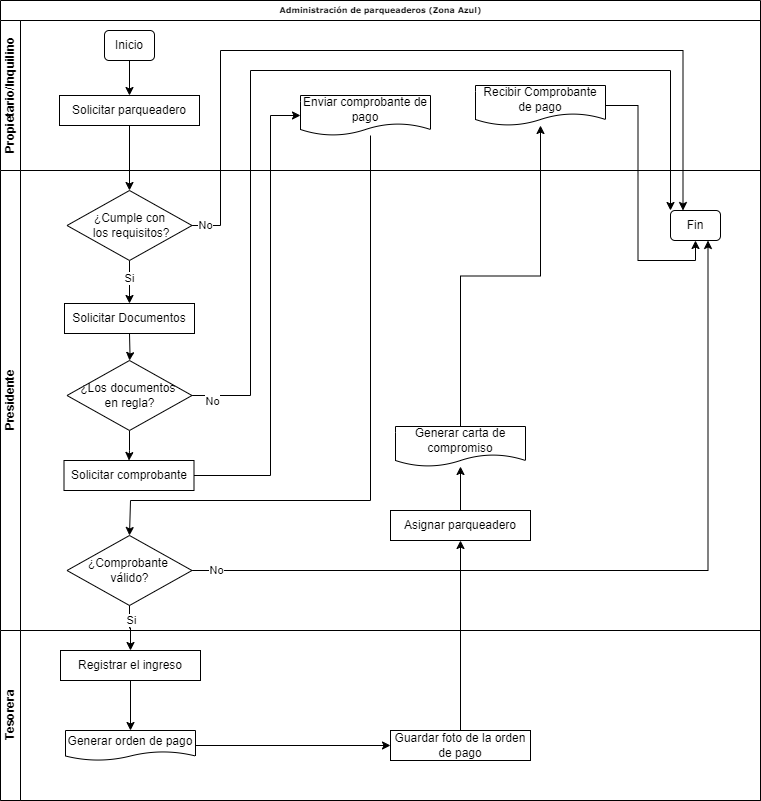
\includegraphics[width=1\textwidth]{resources/images/Diagramade flujo parqueadero-actual}
        \caption{Diagrama de flujo de procesos actual de administración de parqueaderos (Zona azul).}
        \label{fig:flujo-proceso-actual-parqueadero-azul}
    \end{figure}
    \item Proceso de administración de convocatorias.
    \begin{enumerate}
        \item La directiva del conjunto se reúne para definir la fecha de la convocatoria.
        \item Se crea la publicación de la convocatoria y se comparte en los medios de comunicación del conjunto habitacional.
        \item Se reenvía la publicación como recordatoria una semana antes de darse la convocatoria solo si es de asambleas.
        \item Se lleva a cabo la convocatoria.
        \begin{itemize}
            \item Si es una asamblea se procede al siguiente proceso.
            \item Si es una reunión o sesión de directiva se salta al proceso 6.
        \end{itemize}
        \item Se registra la asistencia de los propietarios o inquilinos.
        \item Se tratan los temas de la convocatoria.
        \item Se propone una votación de los temas a tratar.
        \begin{itemize}
            \item Si existe una votación se procede al siguiente proceso.
            \item Si no existe una votación se salta al proceso 9.
        \end{itemize}
        \item Se lleva a cabo el conteo de votos a mano alzada únicamente de propietarios.
        \item Se notifica a los propietarios el resultado de la votación.
        \item Se finaliza la convocatoria.
        \item Se genera el informe de asistencia.
        \item Se genera el acta de la convocatoria.
        \begin{itemize}
            \item Si es una asamblea se procede al siguiente proceso.
            \item Si es una reunión o sesión de directiva se finaliza el proceso.
        \end{itemize}
        \item Se envía el informe de asistencia a los residentes y se registra la respectiva multa.
        \item El propietario o inquilino puede presentar una justificación por la inasistencia en las siguientes 24 horas.
        \item Se verifica la justificación presentada.
        \begin{itemize}
            \item Si la justificación es válida se procede a eliminar la multa y termina el proceso.
            \item Si la justificación no es válida la multa se mantiene y termina el proceso.
        \end{itemize}
    \end{enumerate}

    \begin{figure}[H]
              \centering
              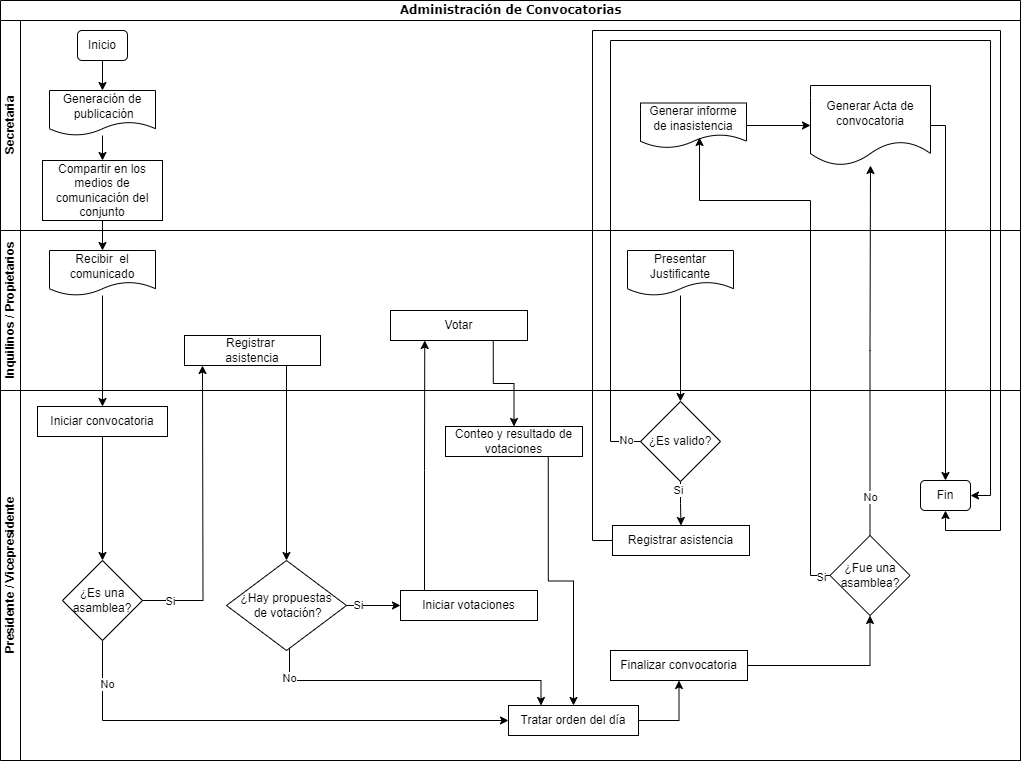
\includegraphics[width=1\textwidth]{resources/images/Copia de Diagrama de flujo convocatorias-actual}
              \caption{Diagrama de flujo de procesos actual de administración de convocatorias.}
              \label{fig:flujo-proceso-actual-convocatorias}
    \end{figure}
    \item Proceso de administración financiera.
    \begin{enumerate}
        \item Pagos de obligaciones financieras mensuales
        \begin{enumerate}
            \item El inquilino realiza el pago de la mensualidad de sus obligaciones financieras.
            \item El inquilino envía el comprobante de pago a la tesorera.
            \item La tesorera verifica el comprobante de pago.
            \begin{itemize}
                \item Si el comprobante es válido se procede al siguiente proceso.
                \item Si el comprobante no es válido se finaliza el proceso.
            \end{itemize}
            \item La tesorera revisa la última fecha de pago del inquilino.
            \item Se registra el pago en el libro de ingresos.
            \item Se genera una orden de pago.
            \item La tesorera entrega la orden de pago a guardianía pára que se le entregue al inquilino.
        \end{enumerate}
        \begin{figure}[H]
            \centering
            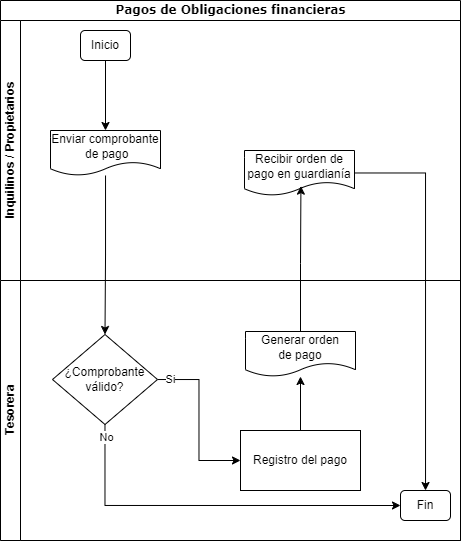
\includegraphics[width=1\textwidth]{resources/images/Diagrama de flujo de proceso pagos obligaciones actual}
            \caption{Diagrama de flujo de procesos actual del pago de obligaciones financieras.}
            \label{fig:flujo-proceso-actual-pagos-obligaciones-financieras}
        \end{figure}
        \item Pagos a proveedores
        \begin{enumerate}
            \item El proveedor envía la factura a la tesorera.
            \item La tesorera verifica la factura.
            \begin{itemize}
                \item Si la factura es válida se procede al siguiente proceso.
                \item Si la factura no es válida se finaliza el proceso.
            \end{itemize}
            \item La tesorera registra la factura en el libro de egresos.
        \end{enumerate}
        \begin{figure}[H]
            \centering
            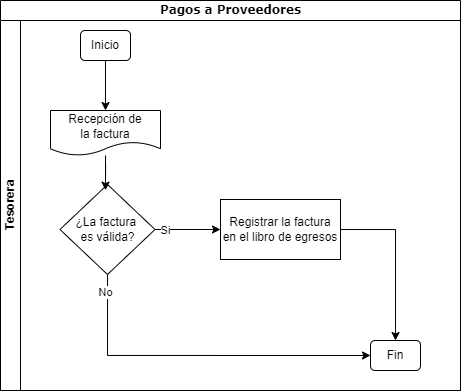
\includegraphics[width=1\textwidth]{resources/images/Diagrama de flujo de proceso pagos a proveedores-actual}
            \caption{Diagrama de flujo de procesos actual del pago de obligaciones financieras.}
            \label{fig:flujo-proceso-actual-pagos-proveedores}
        \end{figure}
        \item Multas
        \begin{enumerate}
            \item Se registra la multa en el libro de multas.
            \item Se guardan mediante fotos en los teléfonos de los directivos las infracciones cometidas por los propietarios o inquilinos.
            \item Se le notifica al propietario o inquilino la multa.
            \item El propietario o inquilino envía el comprobante de pago de la multa.
            \item La tesorera verifica el comprobante de pago.
            \begin{itemize}
                \item Si el comprobante es válido se procede al siguiente proceso.
                \item Si el comprobante no es válido se mantiene la multa y se finaliza el proceso.
            \end{itemize}
            \item Se registra el pago de la multa en el libro de ingresos.
            \item Se genera una orden de pago.
            \item La tesorera entrega la orden de pago a guardianía para que se le entregue al propietario o inquilino.
        \end{enumerate}
        \begin{figure}[H]
            \centering
            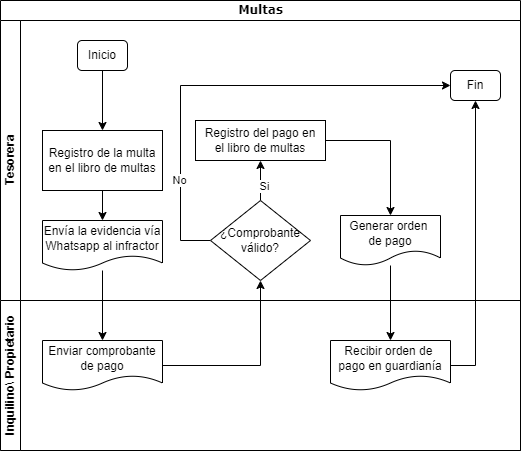
\includegraphics[width=1\textwidth]{resources/images/Diagrama de flujo de proceso multas actual}
            \caption{Diagrama de flujo de procesos actual de multas.}
            \label{fig:flujo-proceso-actual-multas}
        \end{figure}
    \end{enumerate}
\end{itemize}

